% Options for packages loaded elsewhere
\PassOptionsToPackage{unicode}{hyperref}
\PassOptionsToPackage{hyphens}{url}
%
\documentclass[
  brazilian,
]{article}
\usepackage{lmodern}
\usepackage{amssymb,amsmath}
\usepackage{ifxetex,ifluatex}
\ifnum 0\ifxetex 1\fi\ifluatex 1\fi=0 % if pdftex
  \usepackage[T1]{fontenc}
  \usepackage[utf8]{inputenc}
  \usepackage{textcomp} % provide euro and other symbols
\else % if luatex or xetex
  \usepackage{unicode-math}
  \defaultfontfeatures{Scale=MatchLowercase}
  \defaultfontfeatures[\rmfamily]{Ligatures=TeX,Scale=1}
\fi
% Use upquote if available, for straight quotes in verbatim environments
\IfFileExists{upquote.sty}{\usepackage{upquote}}{}
\IfFileExists{microtype.sty}{% use microtype if available
  \usepackage[]{microtype}
  \UseMicrotypeSet[protrusion]{basicmath} % disable protrusion for tt fonts
}{}
\makeatletter
\@ifundefined{KOMAClassName}{% if non-KOMA class
  \IfFileExists{parskip.sty}{%
    \usepackage{parskip}
  }{% else
    \setlength{\parindent}{0pt}
    \setlength{\parskip}{6pt plus 2pt minus 1pt}}
}{% if KOMA class
  \KOMAoptions{parskip=half}}
\makeatother
\usepackage{xcolor}
\IfFileExists{xurl.sty}{\usepackage{xurl}}{} % add URL line breaks if available
\IfFileExists{bookmark.sty}{\usepackage{bookmark}}{\usepackage{hyperref}}
\hypersetup{
  pdftitle={Parte III: Processamento de Linguagem Natural para Linguistas},
  pdfauthor={CiberExt 26-29 · FEELT38103 · Universidade Federal de Uberlândia},
  pdflang={pt-BR},
  hidelinks,
  pdfcreator={LaTeX via pandoc}}
\urlstyle{same} % disable monospaced font for URLs
\usepackage{color}
\usepackage{fancyvrb}
\newcommand{\VerbBar}{|}
\newcommand{\VERB}{\Verb[commandchars=\\\{\}]}
\DefineVerbatimEnvironment{Highlighting}{Verbatim}{commandchars=\\\{\}}
% Add ',fontsize=\small' for more characters per line
\newenvironment{Shaded}{}{}
\newcommand{\AlertTok}[1]{\textcolor[rgb]{1.00,0.00,0.00}{\textbf{#1}}}
\newcommand{\AnnotationTok}[1]{\textcolor[rgb]{0.38,0.63,0.69}{\textbf{\textit{#1}}}}
\newcommand{\AttributeTok}[1]{\textcolor[rgb]{0.49,0.56,0.16}{#1}}
\newcommand{\BaseNTok}[1]{\textcolor[rgb]{0.25,0.63,0.44}{#1}}
\newcommand{\BuiltInTok}[1]{#1}
\newcommand{\CharTok}[1]{\textcolor[rgb]{0.25,0.44,0.63}{#1}}
\newcommand{\CommentTok}[1]{\textcolor[rgb]{0.38,0.63,0.69}{\textit{#1}}}
\newcommand{\CommentVarTok}[1]{\textcolor[rgb]{0.38,0.63,0.69}{\textbf{\textit{#1}}}}
\newcommand{\ConstantTok}[1]{\textcolor[rgb]{0.53,0.00,0.00}{#1}}
\newcommand{\ControlFlowTok}[1]{\textcolor[rgb]{0.00,0.44,0.13}{\textbf{#1}}}
\newcommand{\DataTypeTok}[1]{\textcolor[rgb]{0.56,0.13,0.00}{#1}}
\newcommand{\DecValTok}[1]{\textcolor[rgb]{0.25,0.63,0.44}{#1}}
\newcommand{\DocumentationTok}[1]{\textcolor[rgb]{0.73,0.13,0.13}{\textit{#1}}}
\newcommand{\ErrorTok}[1]{\textcolor[rgb]{1.00,0.00,0.00}{\textbf{#1}}}
\newcommand{\ExtensionTok}[1]{#1}
\newcommand{\FloatTok}[1]{\textcolor[rgb]{0.25,0.63,0.44}{#1}}
\newcommand{\FunctionTok}[1]{\textcolor[rgb]{0.02,0.16,0.49}{#1}}
\newcommand{\ImportTok}[1]{#1}
\newcommand{\InformationTok}[1]{\textcolor[rgb]{0.38,0.63,0.69}{\textbf{\textit{#1}}}}
\newcommand{\KeywordTok}[1]{\textcolor[rgb]{0.00,0.44,0.13}{\textbf{#1}}}
\newcommand{\NormalTok}[1]{#1}
\newcommand{\OperatorTok}[1]{\textcolor[rgb]{0.40,0.40,0.40}{#1}}
\newcommand{\OtherTok}[1]{\textcolor[rgb]{0.00,0.44,0.13}{#1}}
\newcommand{\PreprocessorTok}[1]{\textcolor[rgb]{0.74,0.48,0.00}{#1}}
\newcommand{\RegionMarkerTok}[1]{#1}
\newcommand{\SpecialCharTok}[1]{\textcolor[rgb]{0.25,0.44,0.63}{#1}}
\newcommand{\SpecialStringTok}[1]{\textcolor[rgb]{0.73,0.40,0.53}{#1}}
\newcommand{\StringTok}[1]{\textcolor[rgb]{0.25,0.44,0.63}{#1}}
\newcommand{\VariableTok}[1]{\textcolor[rgb]{0.10,0.09,0.49}{#1}}
\newcommand{\VerbatimStringTok}[1]{\textcolor[rgb]{0.25,0.44,0.63}{#1}}
\newcommand{\WarningTok}[1]{\textcolor[rgb]{0.38,0.63,0.69}{\textbf{\textit{#1}}}}
\usepackage{graphicx}
\makeatletter
\def\maxwidth{\ifdim\Gin@nat@width>\linewidth\linewidth\else\Gin@nat@width\fi}
\def\maxheight{\ifdim\Gin@nat@height>\textheight\textheight\else\Gin@nat@height\fi}
\makeatother
% Scale images if necessary, so that they will not overflow the page
% margins by default, and it is still possible to overwrite the defaults
% using explicit options in \includegraphics[width, height, ...]{}
\setkeys{Gin}{width=\maxwidth,height=\maxheight,keepaspectratio}
% Set default figure placement to htbp
\makeatletter
\def\fps@figure{htbp}
\makeatother
\setlength{\emergencystretch}{3em} % prevent overfull lines
\providecommand{\tightlist}{%
  \setlength{\itemsep}{0pt}\setlength{\parskip}{0pt}}
\setcounter{secnumdepth}{-\maxdimen} % remove section numbering
\ifxetex
  % Load polyglossia as late as possible: uses bidi with RTL langages (e.g. Hebrew, Arabic)
  \usepackage{polyglossia}
  \setmainlanguage[]{brazilian}
\else
  \usepackage[shorthands=off,main=brazilian]{babel}
\fi

\title{Parte III: Processamento de Linguagem Natural para Linguistas}
\usepackage{etoolbox}
\makeatletter
\providecommand{\subtitle}[1]{% add subtitle to \maketitle
  \apptocmd{\@title}{\par {\large #1 \par}}{}{}
}
\makeatother
\subtitle{Unidade 3 - Encontrando padrões linguísticos com o spaCy}
\author{CiberExt 26-29 · FEELT38103 · Universidade Federal de
Uberlândia}
\date{Agosto de 2026}

\begin{document}
\maketitle

\hypertarget{encontrando-padruxf5es-linguuxedsticos-com-o-spacy}{%
\section{Encontrando padrões linguísticos com o
spaCy}\label{encontrando-padruxf5es-linguuxedsticos-com-o-spacy}}

Esta seção ensina você a encontrar padrões linguísticos usando o spaCy,
uma biblioteca de processamento de linguagem natural para Python.

Se você não estiver familiarizado com as anotações linguísticas
produzidas pelo spaCy, ou precisar refrescar a memória, revisite a Parte
II antes de trabalhar nesta seção.

\hypertarget{objetivos-de-aprendizagem}{%
\subsection{Objetivos de Aprendizagem}\label{objetivos-de-aprendizagem}}

Ao final deste módulo, você será capaz de:

\begin{itemize}
\tightlist
\item
  \textbf{Buscar por etiquetas e traços:} Saber como procurar padrões
  com base em etiquetas de classe gramatical (\emph{part-of-speech
  tags}) e traços morfológicos.
\item
  \textbf{Buscar por dependências:} Saber como procurar padrões com base
  em dependências sintáticas.
\item
  \textbf{Examinar o contexto:} Saber como examinar os padrões
  encontrados em seu contexto de ocorrência.
\end{itemize}

\hypertarget{encontrando-padruxf5es-usando-os-matchers-do-spacy}{%
\subsection{\texorpdfstring{1. Encontrando padrões usando os
\emph{Matchers} do
spaCy}{1. Encontrando padrões usando os Matchers do spaCy}}\label{encontrando-padruxf5es-usando-os-matchers-do-spacy}}

Anotações linguísticas, tais como etiquetas de classe gramatical,
dependências sintáticas e traços morfológicos, ajudam a impor estrutura
à linguagem escrita. De maneira crucial, as anotações linguísticas
permitem buscar por \textbf{padrões estruturais} em vez de palavras ou
expressões individuais. Isso permite definir padrões de busca de forma
flexível.

Na biblioteca spaCy, a capacidade de busca por padrões é fornecida por
diversos componentes chamados \emph{Matchers} (algo como ``casadores de
padrões'').

O spaCy oferece três tipos de \emph{Matchers}:

\begin{enumerate}
\def\labelenumi{\arabic{enumi}.}
\tightlist
\item
  O \href{https://spacy.io/api/matcher}{\emph{Matcher}}, que permite
  definir regras que buscam por \textbf{palavras ou expressões}
  específicas examinando os atributos de objetos \emph{Token}.
\item
  O
  \href{https://spacy.io/api/dependencymatcher}{\emph{DependencyMatcher}},
  que permite buscar \textbf{padrões sintáticos} nas árvores de análise.
\item
  O \href{https://spacy.io/api/phrasematcher}{\emph{PhraseMatcher}}, um
  método rápido para casar objetos \emph{Doc} do spaCy com outros
  objetos \emph{Doc}.
\end{enumerate}

As seções a seguir mostram como usar o \emph{Matcher} para casar objetos
\emph{Token} e suas sequências com base em etiquetas de classe
gramatical e traços morfológicos, e como usar o \emph{DependencyMatcher}
para casar dependências sintáticas.

\hypertarget{casando-palavras-ou-expressuxf5es}{%
\subsubsection{1.1. Casando palavras ou
expressões}\label{casando-palavras-ou-expressuxf5es}}

Para começar a trabalhar com o \emph{Matcher}, vamos importar a
biblioteca spaCy e carregar um modelo de linguagem pequeno para o
inglês.

\begin{Shaded}
\begin{Highlighting}[]
\CommentTok{\# Importa a biblioteca spaCy para o Python}
\ImportTok{import}\NormalTok{ spacy}

\CommentTok{\# Carrega um modelo de linguagem pequeno para o inglês; atribui o resultado a \textquotesingle{}nlp\textquotesingle{}}
\NormalTok{nlp }\OperatorTok{=}\NormalTok{ spacy.load(}\StringTok{\textquotesingle{}en\_core\_web\_sm\textquotesingle{}}\NormalTok{)}
\end{Highlighting}
\end{Shaded}

Para termos algum dado com que trabalhar, vamos carregar um texto
extraído de um artigo da Wikipédia.

Para isso, usamos a função \texttt{open()} do Python em combinação com a
instrução \texttt{with} para abrir o arquivo em modo de leitura,
fornecendo os argumentos \texttt{file}, \texttt{mode} e
\texttt{encoding}, conforme instruído na Parte II.

Em seguida, chamamos o método \texttt{read()} para ler o conteúdo do
arquivo e armazenamos o resultado na variável \texttt{text}.

\begin{Shaded}
\begin{Highlighting}[]
\CommentTok{\# Usa a função open() com a instrução \textquotesingle{}with\textquotesingle{} para abrir o arquivo em modo de leitura}
\ControlFlowTok{with} \BuiltInTok{open}\NormalTok{(}\BuiltInTok{file}\OperatorTok{=}\StringTok{\textquotesingle{}data/occupy.txt\textquotesingle{}}\NormalTok{, mode}\OperatorTok{=}\StringTok{\textquotesingle{}r\textquotesingle{}}\NormalTok{, encoding}\OperatorTok{=}\StringTok{\textquotesingle{}utf{-}8\textquotesingle{}}\NormalTok{) }\ImportTok{as} \BuiltInTok{file}\NormalTok{:}

    \CommentTok{\# Usa o método read() para ler o conteúdo do arquivo; atribui o resultado à}
    \CommentTok{\# variável \textquotesingle{}text\textquotesingle{}}
\NormalTok{    text }\OperatorTok{=} \BuiltInTok{file}\NormalTok{.read()}
\end{Highlighting}
\end{Shaded}

Isso devolve um objeto \emph{string} do Python que contém o artigo em
texto puro, agora disponível na variável \texttt{text}.

Em seguida, fornecemos esse objeto ao modelo de linguagem armazenado na
variável \texttt{nlp}, conforme instruído na Parte II.

Também usamos a função \texttt{len()} do Python para contar o número de
palavras no texto.

\begin{Shaded}
\begin{Highlighting}[]
\CommentTok{\# Fornece o objeto string ao modelo de linguagem}
\NormalTok{doc }\OperatorTok{=}\NormalTok{ nlp(text)}

\CommentTok{\# Usa a função len() para verificar o tamanho do objeto Doc e contar}
\CommentTok{\# quantos Tokens estão contidos nele.}
\BuiltInTok{len}\NormalTok{(doc)}
\end{Highlighting}
\end{Shaded}

\begin{verbatim}
14867
\end{verbatim}

Agora que temos um objeto \emph{Doc} do spaCy com quase 15 000
\emph{Tokens}, podemos prosseguir e importar a classe \emph{Matcher} do
submódulo \texttt{matcher} do spaCy.

\begin{Shaded}
\begin{Highlighting}[]
\CommentTok{\# Importa a classe Matcher}
\ImportTok{from}\NormalTok{ spacy.matcher }\ImportTok{import}\NormalTok{ Matcher}
\end{Highlighting}
\end{Shaded}

Importar a classe \emph{Matcher} do submódulo \texttt{matcher} do spaCy
nos permite criar objetos \emph{Matcher}.

Ao criar um objeto \emph{Matcher}, você precisa fornecer a ele o
vocabulário do modelo de linguagem usado para encontrar as
correspondências.

A razão para isso é bastante simples: se você quer buscar padrões em
algum idioma, primeiro precisa conhecer o vocabulário desse idioma.

O spaCy armazena o vocabulário de um modelo em um objeto
\href{https://spacy.io/api/vocab}{\emph{Vocab}}. O objeto \emph{Vocab}
pode ser encontrado no atributo \texttt{vocab} de um objeto
\emph{Language} do spaCy, apresentado na Parte II.

Neste caso, temos o objeto \emph{Language} que contém um modelo de
linguagem pequeno para o inglês armazenado na variável \texttt{nlp}, o
que significa que podemos acessar seu objeto \emph{Vocab} pelo atributo
\texttt{nlp.vocab}.

Chamamos então a \textbf{classe} \emph{Matcher} e fornecemos o
vocabulário disponível em \texttt{nlp.vocab} ao argumento \texttt{vocab}
para criar um objeto \emph{Matcher}. Armazenamos o objeto resultante na
variável \texttt{matcher}.

\begin{Shaded}
\begin{Highlighting}[]
\CommentTok{\# Cria um Matcher e fornece o vocabulário do modelo; atribui o resultado à variável \textquotesingle{}matcher\textquotesingle{}}
\NormalTok{matcher }\OperatorTok{=}\NormalTok{ Matcher(vocab}\OperatorTok{=}\NormalTok{nlp.vocab)}

\CommentTok{\# Chama a variável para examinar o objeto}
\NormalTok{matcher}
\end{Highlighting}
\end{Shaded}

\begin{verbatim}
<spacy.matcher.matcher.Matcher at 0x295de8140>
\end{verbatim}

O objeto \emph{Matcher} está agora pronto para armazenar os padrões que
queremos buscar.

Esses padrões -- ou, mais especificamente, essas \emph{regras de padrão}
-- são criados usando um
\href{https://spacy.io/api/matcher\#patterns}{formato específico}
definido pelo spaCy.

Cada padrão consiste em uma lista Python, que é preenchida por
dicionários Python.

Cada dicionário nessa lista descreve o padrão para casar um único
\emph{Token} do spaCy.

Se você deseja casar uma sequência de \emph{Tokens}, precisa definir
múltiplos dicionários dentro de uma única lista, cuja ordem acompanha a
do padrão a ser casado.

Vamos começar definindo um padrão simples para casar sequências de
pronomes e verbos, e armazenar esse padrão na variável
\texttt{pronoun\_verb}.

Esse padrão consiste em uma lista, marcada pelos colchetes
\texttt{{[}{]}}, que contém dois dicionários, marcados por chaves
\texttt{\{\}} e separados por vírgula. Os pares de chave e valor em um
dicionário são separados por dois-pontos.

\begin{itemize}
\tightlist
\item
  A \textbf{chave} do dicionário determina qual atributo do \emph{Token}
  deve ser buscado. Os atributos suportados pelo \emph{Matcher} podem
  ser encontrados \href{https://spacy.io/api/matcher\#patterns}{aqui}.
\item
  O \textbf{valor} associado à chave determina o valor específico
  daquele atributo.
\end{itemize}

Neste caso, definimos um padrão que busca uma sequência de duas
etiquetas gerais de classe gramatical (\texttt{POS}), apresentadas na
Parte II: pronomes (\texttt{PRON}) e verbos (\texttt{VERB}).

Observe que tanto as chaves quanto os valores devem ser fornecidos em
letras maiúsculas.

\begin{Shaded}
\begin{Highlighting}[]
\CommentTok{\# Define uma lista com dicionários aninhados que contém o padrão a ser casado}
\NormalTok{pronoun\_verb }\OperatorTok{=}\NormalTok{ [\{}\StringTok{\textquotesingle{}POS\textquotesingle{}}\NormalTok{: }\StringTok{\textquotesingle{}PRON\textquotesingle{}}\NormalTok{\}, \{}\StringTok{\textquotesingle{}POS\textquotesingle{}}\NormalTok{: }\StringTok{\textquotesingle{}VERB\textquotesingle{}}\NormalTok{\}]}
\end{Highlighting}
\end{Shaded}

Agora que definimos o padrão usando uma lista e dicionários, podemos
adicioná-lo ao objeto \emph{Matcher} armazenado na variável
\texttt{matcher}.

Isso pode ser feito com o método \texttt{add()}, que exige duas
entradas:

\begin{enumerate}
\def\labelenumi{\arabic{enumi}.}
\tightlist
\item
  Um objeto \emph{string} do Python que define um nome para o padrão.
  Isso é necessário para fins de identificação.
\item
  Uma lista contendo o(s) padrão(ões) a ser(em) buscado(s). Como uma
  única regra de casamento de padrões pode conter múltiplos padrões, a
  entrada deve ser uma \emph{lista de listas}. Por isso envolvemos as
  listas de entrada em colchetes, por exemplo \texttt{{[}pattern\_1{]}}.
\end{enumerate}

\begin{Shaded}
\begin{Highlighting}[]
\CommentTok{\# Adiciona o padrão ao matcher sob o nome \textquotesingle{}pronoun+verb\textquotesingle{}}
\NormalTok{matcher.add(}\StringTok{"pronoun+verb"}\NormalTok{, patterns}\OperatorTok{=}\NormalTok{[pronoun\_verb])}
\end{Highlighting}
\end{Shaded}

Para buscar correspondências no objeto \emph{Doc} armazenado na variável
\texttt{doc}, fornecemos o objeto \emph{Doc} ao \emph{Matcher} e
armazenamos o resultado na variável \texttt{result}.

Também definimos o argumento opcional \texttt{as\_spans} como
\texttt{True}, o que instrui o spaCy a devolver os resultados como
objetos \emph{Span}.

Como você deve lembrar da Parte II, objetos \emph{Span} correspondem a
``fatias'' contínuas de objetos \emph{Doc}.

\begin{Shaded}
\begin{Highlighting}[]
\CommentTok{\# Aplica o Matcher ao objeto Doc armazenado em \textquotesingle{}doc\textquotesingle{}; fornece o argumento}
\CommentTok{\# \textquotesingle{}as\_spans\textquotesingle{} com o valor True para obter Spans como saída}
\NormalTok{result }\OperatorTok{=}\NormalTok{ matcher(doc, as\_spans}\OperatorTok{=}\VariableTok{True}\NormalTok{)}

\CommentTok{\# Chama a variável para examinar a saída}
\NormalTok{result}
\end{Highlighting}
\end{Shaded}

\begin{verbatim}
[that expressed,
 It aimed,
 It formed,
 this began,
 it organizes,
 that read,
 who designed,
 He wrote,
 there were,
 They promoted,
 It refers,
 which started,
 that indicate,
 that allowed,
 they saw,
 they argued,
 they called,
 it takes,
 ...
 that deals,
 that believe]
\end{verbatim}

A saída é uma lista de objetos \emph{Span} do spaCy que casam com o
padrão solicitado. Vamos examinar o primeiro objeto da lista de
correspondências em maior detalhe.

\begin{Shaded}
\begin{Highlighting}[]
\NormalTok{result[}\DecValTok{0}\NormalTok{]}
\end{Highlighting}
\end{Shaded}

\begin{verbatim}
that expressed
\end{verbatim}

O objeto \emph{Span} possui vários
\href{https://spacy.io/api/span}{atributos} úteis, entre eles
\texttt{start} e \texttt{end}. Esses atributos contêm os índices que
indicam onde, no objeto \emph{Doc}, o \emph{Span} começa e termina.

\begin{Shaded}
\begin{Highlighting}[]
\NormalTok{result[}\DecValTok{0}\NormalTok{].start, result[}\DecValTok{0}\NormalTok{].end}
\end{Highlighting}
\end{Shaded}

\begin{verbatim}
(14, 16)
\end{verbatim}

Outro atributo útil é o \texttt{label}, que contém o nome que demos ao
padrão. Vamos observá-lo mais de perto.

\begin{Shaded}
\begin{Highlighting}[]
\NormalTok{result[}\DecValTok{0}\NormalTok{].label}
\end{Highlighting}
\end{Shaded}

\begin{verbatim}
12298179334642351811
\end{verbatim}

O número armazenado no atributo \texttt{label} é, na verdade, um objeto
\href{https://spacy.io/api/lexeme}{\emph{Lexeme}} do spaCy, que
corresponde a uma entrada no vocabulário do modelo de linguagem.

Esse \emph{Lexeme} contém o nome que demos ao padrão de busca acima, ou
seja, \texttt{pronoun+verb}.

Podemos verificar isso facilmente usando o valor de
\texttt{result{[}0{]}.label} para buscar o \emph{Lexeme} no objeto
\emph{Vocab} disponível em \texttt{nlp.vocab} e examinando seu atributo
\texttt{text}.

\begin{Shaded}
\begin{Highlighting}[]
\CommentTok{\# Acessa o vocabulário do modelo usando colchetes; fornece o valor de \textquotesingle{}result[0].label\textquotesingle{}}
\CommentTok{\# como chave. Em seguida, obtém o atributo \textquotesingle{}text\textquotesingle{} do objeto Lexeme, que contém o}
\CommentTok{\# lexema em forma legível para humanos.}
\NormalTok{nlp.vocab[result[}\DecValTok{0}\NormalTok{].label].text}
\end{Highlighting}
\end{Shaded}

\begin{verbatim}
'pronoun+verb'
\end{verbatim}

A informação disponível no atributo \texttt{label} é útil para
desambiguar entre padrões, especialmente se o mesmo objeto
\emph{Matcher} contiver vários padrões diferentes, como veremos logo
adiante.

Olhando para as correspondências acima, o padrão que definimos é
bastante restritivo, pois o pronome e o verbo precisam vir imediatamente
um após o outro.

Não conseguimos, por exemplo, casar padrões em que o verbo é precedido
por verbos auxiliares.

O spaCy permite aumentar a flexibilidade das regras de padrão por meio
de \textbf{operadores}.

Esses operadores são definidos adicionando a chave \texttt{OP} ao
dicionário que define o padrão de um único \emph{Token}. O spaCy suporta
os seguintes operadores:

\begin{itemize}
\tightlist
\item
  \texttt{!}: Nega o padrão; o padrão pode ocorrer exatamente zero
  vezes.
\item
  \texttt{?}: Torna o padrão opcional; o padrão pode ocorrer zero ou uma
  vez.
\item
  \texttt{+}: Exige que o padrão ocorra uma ou mais vezes.
\item
  \texttt{*}: Permite que o padrão ocorra zero ou mais vezes.
\end{itemize}

Vamos explorar o uso de operadores definindo outra regra de padrão, que
amplia o alcance do nosso \emph{Matcher}.

Para tanto, definimos um padrão adicional para um \emph{Token} entre o
pronome e o verbo. Esse \emph{Token} deve ter a etiqueta geral de classe
gramatical \texttt{AUX}, que indica um verbo auxiliar:

\begin{Shaded}
\begin{Highlighting}[]
\NormalTok{\{}\StringTok{\textquotesingle{}POS\textquotesingle{}}\NormalTok{: }\StringTok{\textquotesingle{}AUX\textquotesingle{}}\NormalTok{, }\StringTok{\textquotesingle{}OP\textquotesingle{}}\NormalTok{: }\StringTok{\textquotesingle{}+\textquotesingle{}}\NormalTok{\}}
\end{Highlighting}
\end{Shaded}

Além disso, acrescentamos outro par de chave e valor ao dicionário desse
\emph{Token}, contendo a chave \texttt{OP} com o valor \texttt{+}. Isso
significa que o \emph{Token} correspondente a um verbo auxiliar deve
ocorrer \emph{uma ou mais vezes}.

Armazenamos a lista resultante com dicionários aninhados na variável
\texttt{pronoun\_aux\_verb} e adicionamos o padrão ao objeto
\emph{Matcher} já existente, armazenado na variável \texttt{matcher}.

\begin{Shaded}
\begin{Highlighting}[]
\CommentTok{\# Define uma lista com dicionários aninhados que contém o padrão a ser casado}
\NormalTok{pronoun\_aux\_verb }\OperatorTok{=}\NormalTok{ [\{}\StringTok{\textquotesingle{}POS\textquotesingle{}}\NormalTok{: }\StringTok{\textquotesingle{}PRON\textquotesingle{}}\NormalTok{\}, \{}\StringTok{\textquotesingle{}POS\textquotesingle{}}\NormalTok{: }\StringTok{\textquotesingle{}AUX\textquotesingle{}}\NormalTok{, }\StringTok{\textquotesingle{}OP\textquotesingle{}}\NormalTok{: }\StringTok{\textquotesingle{}+\textquotesingle{}}\NormalTok{\}, \{}\StringTok{\textquotesingle{}POS\textquotesingle{}}\NormalTok{: }\StringTok{\textquotesingle{}VERB\textquotesingle{}}\NormalTok{\}]}

\CommentTok{\# Adiciona o padrão ao matcher sob o nome \textquotesingle{}pronoun+aux+verb\textquotesingle{}}
\NormalTok{matcher.add(}\StringTok{\textquotesingle{}pronoun+aux+verb\textquotesingle{}}\NormalTok{, patterns}\OperatorTok{=}\NormalTok{[pronoun\_aux\_verb])}

\CommentTok{\# Aplica o Matcher ao objeto Doc armazenado em \textquotesingle{}doc\textquotesingle{}; fornece o argumento \textquotesingle{}as\_spans\textquotesingle{}}
\CommentTok{\# com o valor True para obter Spans como saída. Sobrescreve as correspondências}
\CommentTok{\# anteriores armazenando o resultado na variável \textquotesingle{}results\textquotesingle{}.}
\NormalTok{results }\OperatorTok{=}\NormalTok{ matcher(doc, as\_spans}\OperatorTok{=}\VariableTok{True}\NormalTok{)}
\end{Highlighting}
\end{Shaded}

Assim como antes, o \emph{Matcher} devolve uma lista de objetos
\emph{Span} do spaCy.

Vamos percorrer cada item da lista \texttt{results}. Usamos a variável
\texttt{result} para nos referirmos aos objetos \emph{Span} individuais
da lista, que contêm nossas correspondências.

Primeiro recuperamos o objeto \emph{Lexeme} armazenado em
\texttt{result.label}, que mapeamos para o \emph{Vocabulário} do modelo
de linguagem disponível em \texttt{nlp.vocab}.

Como aprendemos acima, esse \emph{Lexeme} corresponde ao nome que demos
à regra de padrão, cuja forma legível para humanos pode ser encontrada
no atributo \texttt{text}.

Em seguida, imprimimos um caractere de tabulação para inserir algum
espaço entre o nome do padrão e o objeto \emph{Span} que contém a
correspondência.

\begin{Shaded}
\begin{Highlighting}[]
\CommentTok{\# Percorre cada objeto Span na lista \textquotesingle{}results\textquotesingle{}}
\ControlFlowTok{for}\NormalTok{ result }\KeywordTok{in}\NormalTok{ results:}

    \CommentTok{\# Imprime o nome da regra de padrão, um caractere de tabulação e o Span correspondente}
    \BuiltInTok{print}\NormalTok{(nlp.vocab[result.label].text, }\StringTok{\textquotesingle{}}\CharTok{\textbackslash{}t}\StringTok{\textquotesingle{}}\NormalTok{, result)}
\end{Highlighting}
\end{Shaded}

\begin{verbatim}
pronoun+verb     that expressed
pronoun+verb     It aimed
pronoun+verb     It formed
pronoun+verb     this began
pronoun+verb     it organizes
pronoun+aux+verb     that had resulted
pronoun+verb     that read
pronoun+verb     who designed
pronoun+verb     He wrote
pronoun+verb     there were
pronoun+aux+verb     they did have
pronoun+verb     they saw
pronoun+aux+verb     they were working
pronoun+aux+verb     which has been gathered
pronoun+aux+verb     who had lost
pronoun+aux+verb     that can be traced
...
pronoun+aux+verb     they have been protesting
pronoun+aux+verb     they will have made
pronoun+aux+verb     which would overturn
pronoun+verb     that believe
\end{verbatim}

A saída mostra que o padrão que adicionamos ao \emph{Matcher} casa com
padrões que contêm um (por exemplo, ``we \emph{can} build'') ou mais
(por exemplo, ``they \emph{have been} protesting'') auxiliares!

\hypertarget{casando-trauxe7os-morfoluxf3gicos}{%
\subsubsection{1.2. Casando traços
morfológicos}\label{casando-trauxe7os-morfoluxf3gicos}}

Como apresentado na Parte II, o spaCy também pode realizar análise
morfológica, cujos resultados são armazenados no atributo \texttt{morph}
de um objeto \emph{Token}.

O atributo \texttt{morph} contém um objeto \emph{string}, no qual cada
traço morfológico é separado por uma barra vertical \texttt{\textbar{}},
como ilustrado abaixo.

\begin{verbatim}
We   Case=Nom|Number=Plur|Person=1|PronType=Prs
\end{verbatim}

Como você pode ver, os tipos específicos de traços morfológicos -- por
exemplo, \emph{Case} (caso) -- e seu valor -- por exemplo, \emph{Nom}
(para o caso nominativo) -- são separados por sinais de igual
\texttt{=}.

Vamos começar a explorar como podemos definir regras de padrão que casam
traços morfológicos.

Para começar, criamos um novo objeto \emph{Matcher} chamado
\texttt{morph\_matcher}.

\begin{Shaded}
\begin{Highlighting}[]
\CommentTok{\# Cria um Matcher e fornece o vocabulário do modelo; atribui o resultado à variável \textquotesingle{}morph\_matcher\textquotesingle{}}
\NormalTok{morph\_matcher }\OperatorTok{=}\NormalTok{ Matcher(vocab}\OperatorTok{=}\NormalTok{nlp.vocab)}
\end{Highlighting}
\end{Shaded}

Definimos então um novo padrão com regras para dois \emph{Tokens}:

\begin{enumerate}
\def\labelenumi{\arabic{enumi}.}
\tightlist
\item
  \emph{Tokens} que possuem a etiqueta refinada de classe gramatical
  \texttt{NNP} (nome próprio), que pode ocorrer uma ou mais vezes
  (operador: \texttt{+}).
\end{enumerate}

\begin{Shaded}
\begin{Highlighting}[]
\NormalTok{\{}\StringTok{\textquotesingle{}TAG\textquotesingle{}}\NormalTok{: }\StringTok{\textquotesingle{}NNP\textquotesingle{}}\NormalTok{, }\StringTok{\textquotesingle{}OP\textquotesingle{}}\NormalTok{: }\StringTok{\textquotesingle{}+\textquotesingle{}}\NormalTok{\}}
\end{Highlighting}
\end{Shaded}

\begin{enumerate}
\def\labelenumi{\arabic{enumi}.}
\setcounter{enumi}{1}
\tightlist
\item
  \emph{Tokens} que possuem a etiqueta geral de classe gramatical
  \texttt{VERB} e que apresentam \emph{todos} os seguintes traços
  morfológicos (\texttt{MORPH}):
  \texttt{Number=Sing\textbar{}Person=Three\textbar{}Tense=Pres\textbar{}VerbForm=Fin}.
\end{enumerate}

\begin{Shaded}
\begin{Highlighting}[]
\NormalTok{\{}\StringTok{\textquotesingle{}POS\textquotesingle{}}\NormalTok{: }\StringTok{\textquotesingle{}VERB\textquotesingle{}}\NormalTok{, }\StringTok{\textquotesingle{}MORPH\textquotesingle{}}\NormalTok{: }\StringTok{\textquotesingle{}Number=Sing|Person=Three|Tense=Pres|VerbForm=Fin\textquotesingle{}}\NormalTok{\}}
\end{Highlighting}
\end{Shaded}

Definimos o padrão usando dois dicionários em uma lista, que atribuímos
à variável \texttt{propn\_3rd\_finite}.

\begin{Shaded}
\begin{Highlighting}[]
\CommentTok{\# Define uma lista com dicionários aninhados que contém o padrão a ser casado}
\NormalTok{propn\_3rd\_finite }\OperatorTok{=}\NormalTok{ [\{}\StringTok{\textquotesingle{}TAG\textquotesingle{}}\NormalTok{: }\StringTok{\textquotesingle{}NNP\textquotesingle{}}\NormalTok{, }\StringTok{\textquotesingle{}OP\textquotesingle{}}\NormalTok{: }\StringTok{\textquotesingle{}+\textquotesingle{}}\NormalTok{\},}
\NormalTok{                    \{}\StringTok{\textquotesingle{}POS\textquotesingle{}}\NormalTok{: }\StringTok{\textquotesingle{}VERB\textquotesingle{}}\NormalTok{, }\StringTok{\textquotesingle{}MORPH\textquotesingle{}}\NormalTok{: }\StringTok{\textquotesingle{}Number=Sing|Person=Three|Tense=Pres|VerbForm=Fin\textquotesingle{}}\NormalTok{\}]}
\end{Highlighting}
\end{Shaded}

Em seguida, adicionamos o padrão ao \emph{Matcher} recém-criado,
armazenado na variável \texttt{morph\_matcher}, usando o método
\texttt{add()}.

Também fornecemos o valor \texttt{LONGEST} ao argumento opcional
\texttt{greedy} do método \texttt{add()}.

O argumento \texttt{greedy} filtra as correspondências para
\emph{Tokens} que incluem operadores como o \texttt{+}, que buscam de
forma \emph{gulosa} mais de uma correspondência.

Ao definir o valor como \texttt{LONGEST}, o spaCy devolve a sequência
mais longa de correspondências, em vez de devolver uma correspondência a
cada vez que encontra uma. Em outras palavras, o spaCy coletará todos os
\emph{Tokens} correspondentes antes de devolvê-los.

\begin{Shaded}
\begin{Highlighting}[]
\CommentTok{\# Adiciona o padrão ao matcher sob o nome \textquotesingle{}sing\_3rd\_pres\_fin\textquotesingle{}}
\NormalTok{morph\_matcher.add(}\StringTok{\textquotesingle{}sing\_3rd\_pres\_fin\textquotesingle{}}\NormalTok{, patterns}\OperatorTok{=}\NormalTok{[propn\_3rd\_finite], greedy}\OperatorTok{=}\StringTok{\textquotesingle{}LONGEST\textquotesingle{}}\NormalTok{)}
\end{Highlighting}
\end{Shaded}

Aplicamos então o \emph{Matcher} aos dados armazenados na variável
\texttt{doc}.

\begin{Shaded}
\begin{Highlighting}[]
\CommentTok{\# Aplica o Matcher ao objeto Doc armazenado em \textquotesingle{}doc\textquotesingle{}; fornece o argumento \textquotesingle{}as\_spans\textquotesingle{}}
\CommentTok{\# com o valor True para obter Spans como saída. Sobrescreve as correspondências}
\CommentTok{\# anteriores armazenando o resultado na variável \textquotesingle{}morph\_results\textquotesingle{}.}
\NormalTok{morph\_results }\OperatorTok{=}\NormalTok{ morph\_matcher(doc, as\_spans}\OperatorTok{=}\VariableTok{True}\NormalTok{)}

\CommentTok{\# Percorre cada objeto Span na lista \textquotesingle{}morph\_results\textquotesingle{}}
\ControlFlowTok{for}\NormalTok{ result }\KeywordTok{in}\NormalTok{ morph\_results:}

    \CommentTok{\# Imprime o resultado}
    \BuiltInTok{print}\NormalTok{(result)}
\end{Highlighting}
\end{Shaded}

Como você pode ver, as correspondências são relativamente poucas, porque
definimos que o verbo deveria ter traços morfológicos bastante
específicos.

A questão, então, é: como podemos casar apenas \emph{alguns} traços
morfológicos?

Para afrouxar os critérios relativos aos traços morfológicos,
concentrando-nos apenas no
\href{https://pt.wikipedia.org/wiki/Tempo_(gram\%C3\%A1tica)}{tempo
verbal}, precisamos usar um dicionário com a chave \texttt{MORPH}, mas,
em vez de um objeto \emph{string}, fornecemos um dicionário como valor.

Para esse dicionário, usamos a \emph{string} \texttt{IS\_SUPERSET} como
chave. \texttt{IS\_SUPERSET} é um dos atributos definidos no
\href{https://spacy.io/api/matcher\#patterns}{formato de padrões} do
spaCy, por exemplo:

\begin{Shaded}
\begin{Highlighting}[]
\NormalTok{\{}\StringTok{\textquotesingle{}MORPH\textquotesingle{}}\NormalTok{: \{}\StringTok{\textquotesingle{}IS\_SUPERSET\textquotesingle{}}\NormalTok{: [...]\}\}}
\end{Highlighting}
\end{Shaded}

Antes de prosseguirmos, vamos desempacotar um pouco a lógica por trás do
\texttt{IS\_SUPERSET}.

Podemos pensar nos traços morfológicos associados a um dado \emph{Token}
como um \href{https://pt.wikipedia.org/wiki/Conjunto}{conjunto}. Para
exemplificar, um conjunto poderia consistir nos seguintes quatro itens:

\begin{verbatim}
Number=Sing, Person=Three, Tense=Pres, VerbForm=Fin
\end{verbatim}

Se tivéssemos \emph{outro conjunto} com apenas um item,
\texttt{Tense=Pres}, poderíamos descrever a relação entre os dois
conjuntos afirmando que o primeiro conjunto (com quatro itens) é um
\textbf{superconjunto} do segundo (com um item).

Em outras palavras, o conjunto maior (superconjunto) contém o conjunto
menor (subconjunto).

É assim também que funciona o casamento por meio de
\texttt{IS\_SUPERSET}: o spaCy recupera os traços morfológicos de cada
\emph{Token} e verifica se esses traços formam um superconjunto dos
traços definidos no padrão de busca.

Os traços morfológicos a serem buscados são fornecidos como uma lista de
\emph{strings} do Python.

Essas \emph{strings}, por sua vez, definem traços morfológicos
específicos, como \texttt{Tense=Past}, conforme definido no esquema de
\href{https://universaldependencies.org/u/overview/morphology.html}{Dependências
Universais} para a descrição da morfologia, apresentado na unidade
anterior.

Essa lista é então usada como valor da chave \texttt{IS\_SUPERSET}.

Vamos agora buscar verbos no passado e adicioná-los ao objeto
\emph{Matcher} armazenado em \texttt{morph\_matcher}.

\begin{Shaded}
\begin{Highlighting}[]
\CommentTok{\# Define uma lista com dicionários aninhados que contém o padrão a ser casado}
\NormalTok{past\_tense }\OperatorTok{=}\NormalTok{ [\{}\StringTok{\textquotesingle{}TAG\textquotesingle{}}\NormalTok{: }\StringTok{\textquotesingle{}NNP\textquotesingle{}}\NormalTok{, }\StringTok{\textquotesingle{}OP\textquotesingle{}}\NormalTok{: }\StringTok{\textquotesingle{}+\textquotesingle{}}\NormalTok{\},}
\NormalTok{              \{}\StringTok{\textquotesingle{}POS\textquotesingle{}}\NormalTok{: }\StringTok{\textquotesingle{}VERB\textquotesingle{}}\NormalTok{, }\StringTok{\textquotesingle{}MORPH\textquotesingle{}}\NormalTok{: \{}\StringTok{\textquotesingle{}IS\_SUPERSET\textquotesingle{}}\NormalTok{: [}\StringTok{\textquotesingle{}Tense=Past\textquotesingle{}}\NormalTok{]\}\}]}

\CommentTok{\# Adiciona o padrão ao matcher sob o nome \textquotesingle{}past\_tense\textquotesingle{}}
\NormalTok{morph\_matcher.add(}\StringTok{\textquotesingle{}past\_tense\textquotesingle{}}\NormalTok{, patterns}\OperatorTok{=}\NormalTok{[past\_tense], greedy}\OperatorTok{=}\StringTok{\textquotesingle{}LONGEST\textquotesingle{}}\NormalTok{)}

\CommentTok{\# Aplica o Matcher ao objeto Doc armazenado em \textquotesingle{}doc\textquotesingle{}; fornece o argumento \textquotesingle{}as\_spans\textquotesingle{}}
\CommentTok{\# com o valor True para obter Spans como saída. Sobrescreve as correspondências}
\CommentTok{\# anteriores armazenando o resultado na variável \textquotesingle{}morph\_results\textquotesingle{}.}
\NormalTok{morph\_results }\OperatorTok{=}\NormalTok{ morph\_matcher(doc, as\_spans}\OperatorTok{=}\VariableTok{True}\NormalTok{)}
\end{Highlighting}
\end{Shaded}

Vamos percorrer os resultados e imprimir o nome do padrão, o objeto
\emph{Span} que contém a correspondência e os traços morfológicos do
último \emph{Token} da correspondência, que corresponde ao verbo.

\begin{Shaded}
\begin{Highlighting}[]
\CommentTok{\# Percorre cada objeto Span na lista \textquotesingle{}morph\_results\textquotesingle{}}
\ControlFlowTok{for}\NormalTok{ result }\KeywordTok{in}\NormalTok{ morph\_results:}

    \CommentTok{\# Imprime o nome da regra de padrão, um caractere de tabulação e o Span}
    \CommentTok{\# correspondente. Por fim, imprime outro caractere de tabulação, seguido dos}
    \CommentTok{\# traços morfológicos do último Token da correspondência (um verbo).}
    \BuiltInTok{print}\NormalTok{(nlp.vocab[result.label].text, }\StringTok{\textquotesingle{}}\CharTok{\textbackslash{}t}\StringTok{\textquotesingle{}}\NormalTok{, result, }\StringTok{\textquotesingle{}}\CharTok{\textbackslash{}t}\StringTok{\textquotesingle{}}\NormalTok{, result[}\OperatorTok{{-}}\DecValTok{1}\NormalTok{].morph)}
\end{Highlighting}
\end{Shaded}

\begin{verbatim}
past_tense   Community Environmental Legal Defense Fund released     Tense=Past|VerbForm=Fin
past_tense   Oakland Police Chief Howard Jordan expressed    Tense=Past|VerbForm=Fin
past_tense   U.S. Vice President Al Gore called      Tense=Past|VerbForm=Fin
past_tense   Los Angeles City Council became     Tense=Past|VerbForm=Fin
past_tense   Judge Jed S. Rakoff sided   Tense=Past|VerbForm=Fin
past_tense   Prime Minister Manmohan Singh described     Tense=Past|VerbForm=Fin
past_tense   New York Times reported     Tense=Past|VerbForm=Fin
...
past_tense   United Nations controlled   Aspect=Perf|Tense=Past|VerbForm=Part
past_tense   Occupy Glasgow set      Aspect=Perf|Tense=Past|VerbForm=Part
past_tense   Shapiro filed   Tense=Past|VerbForm=Fin
\end{verbatim}

Como você pode ver, o padrão \texttt{past\_tense} consegue casar objetos
com base em um único traço morfológico, embora a maioria das
correspondências compartilhe também outro traço morfológico, a saber, a
forma finita.

\hypertarget{casando-dependuxeancias-sintuxe1ticas}{%
\subsubsection{1.3. Casando dependências
sintáticas}\label{casando-dependuxeancias-sintuxe1ticas}}

Se você quiser casar padrões com base em dependências sintáticas,
precisa usar a classe \emph{DependencyMatcher} do spaCy.

Como aprendemos na Parte II, dependências sintáticas descrevem as
relações que se mantêm entre objetos \emph{Token}.

Para começar, vamos importar a classe \emph{DependencyMatcher} do
submódulo \texttt{matcher}.

Como você pode ver, o \emph{DependencyMatcher} é inicializado exatamente
como o \emph{Matcher} acima.

\begin{Shaded}
\begin{Highlighting}[]
\CommentTok{\# Importa a classe DependencyMatcher}
\ImportTok{from}\NormalTok{ spacy.matcher }\ImportTok{import}\NormalTok{ DependencyMatcher}

\CommentTok{\# Cria um DependencyMatcher e fornece o vocabulário do modelo;}
\CommentTok{\# atribui o resultado à variável \textquotesingle{}dep\_matcher\textquotesingle{}}
\NormalTok{dep\_matcher }\OperatorTok{=}\NormalTok{ DependencyMatcher(vocab}\OperatorTok{=}\NormalTok{nlp.vocab)}
\end{Highlighting}
\end{Shaded}

Isso nos fornece um \emph{DependencyMatcher} armazenado na variável
\texttt{dep\_matcher}, que está agora pronto para armazenar padrões de
dependência.

Ao desenvolver regras de padrão para casar dependências sintáticas, o
primeiro passo é determinar uma \textbf{``âncora''} em torno da qual o
padrão é construído.

Visualizar as dependências sintáticas, como instruído na Parte II, pode
ajudar a formular os padrões.

Vamos importar o submódulo \texttt{displacy} para desenhar as
dependências sintáticas de uma sentença do objeto \emph{Doc} armazenado
na variável \texttt{doc}.

\begin{Shaded}
\begin{Highlighting}[]
\CommentTok{\# Importa o submódulo displacy do spaCy}
\ImportTok{from}\NormalTok{ spacy }\ImportTok{import}\NormalTok{ displacy}

\CommentTok{\# Converte as sentenças contidas no objeto Doc em uma lista; toma a sentença}
\CommentTok{\# no índice 420. Define o atributo \textquotesingle{}style\textquotesingle{} como \textquotesingle{}dep\textquotesingle{} para desenhar as}
\CommentTok{\# dependências sintáticas.}
\NormalTok{displacy.render(}\BuiltInTok{list}\NormalTok{(doc.sents)[}\DecValTok{420}\NormalTok{], style}\OperatorTok{=}\StringTok{\textquotesingle{}dep\textquotesingle{}}\NormalTok{)}
\end{Highlighting}
\end{Shaded}

\begin{figure}
\centering
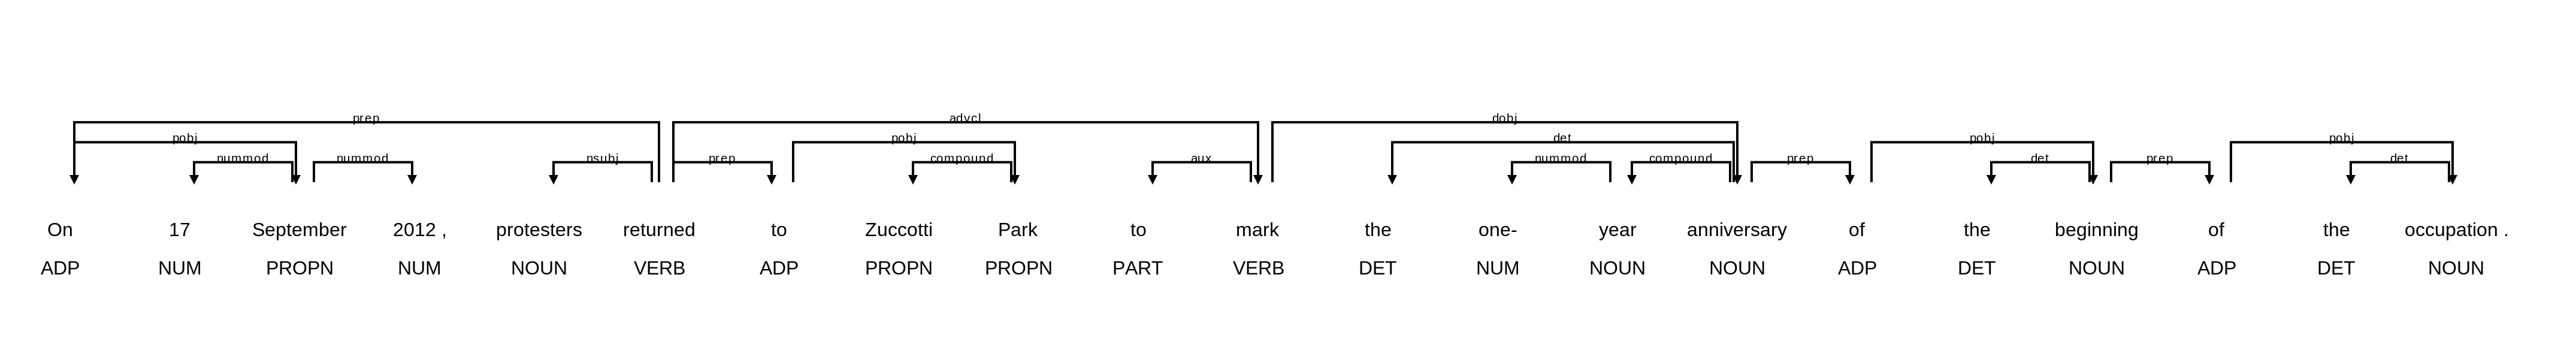
\includegraphics{../resources/image11.png}
\caption{Imagem11}
\end{figure}

Como apresentado na unidade anterior, as dependências sintáticas são
visualizadas por meio de arcos que partem do \emph{Token}
\textbf{cabeça} em direção ao \emph{Token} \textbf{dependente}. O rótulo
do arco indica a dependência sintática.

Vamos definir um padrão que busque verbos e seus sujeitos nominais
(\texttt{nsubj}).

Assim como no caso da classe \emph{Matcher}, as regras de padrão do
\emph{DependencyMatcher} são definidas usando uma lista de dicionários.

O primeiro dicionário da lista define o padrão ``âncora'' e seus
atributos.

Você pode pensar na regra de padrão como uma corrente que avança da
esquerda para a direita, na qual o primeiro padrão à esquerda funciona
como âncora para os padrões subsequentes à sua direita.

Assim, definimos o seguinte padrão para a âncora:

\begin{Shaded}
\begin{Highlighting}[]
\NormalTok{\{}\StringTok{\textquotesingle{}RIGHT\_ID\textquotesingle{}}\NormalTok{: }\StringTok{\textquotesingle{}verb\textquotesingle{}}\NormalTok{, }\StringTok{\textquotesingle{}RIGHT\_ATTRS\textquotesingle{}}\NormalTok{: \{}\StringTok{\textquotesingle{}POS\textquotesingle{}}\NormalTok{: }\StringTok{\textquotesingle{}VERB\textquotesingle{}}\NormalTok{\}\}}
\end{Highlighting}
\end{Shaded}

Usamos a chave obrigatória \texttt{RIGHT\_ID} para fornecer um nome a
esse padrão, que poderá então ser usado para referenciá-lo a partir de
padrões posicionados à sua \textbf{direita}.

Em outras palavras, quando você vir a chave \texttt{RIGHT\_ID}, pense em
um nome para o \emph{padrão atual}.

Criamos então um dicionário sob a chave \texttt{RIGHT\_ATTRS} que guarda
os traços linguísticos da âncora. Neste caso, determinamos que a âncora
deve ter \texttt{VERB} como etiqueta de classe gramatical.

Em seguida, determinamos um padrão para o próximo ``elo'' da corrente, à
direita da âncora:

\begin{Shaded}
\begin{Highlighting}[]
\NormalTok{\{}\StringTok{\textquotesingle{}LEFT\_ID\textquotesingle{}}\NormalTok{: }\StringTok{\textquotesingle{}verb\textquotesingle{}}\NormalTok{, }\StringTok{\textquotesingle{}REL\_OP\textquotesingle{}}\NormalTok{: }\StringTok{\textquotesingle{}\textgreater{}\textquotesingle{}}\NormalTok{, }\StringTok{\textquotesingle{}RIGHT\_ID\textquotesingle{}}\NormalTok{: }\StringTok{\textquotesingle{}subject\textquotesingle{}}\NormalTok{, }\StringTok{\textquotesingle{}RIGHT\_ATTRS\textquotesingle{}}\NormalTok{: \{}\StringTok{\textquotesingle{}DEP\textquotesingle{}}\NormalTok{: }\StringTok{\textquotesingle{}nsubj\textquotesingle{}}\NormalTok{\}\}}
\end{Highlighting}
\end{Shaded}

Começamos fornecendo a chave \texttt{LEFT\_ID}, cujo valor é um objeto
\emph{string} que se refere ao nome de um padrão à \textbf{esquerda} do
padrão atual. Esse é o nome que demos à âncora usando a chave
\texttt{RIGHT\_ID}.

Em seguida, usamos a chave \texttt{REL\_OP} para definir um
\href{https://spacy.io/api/dependencymatcher\#patterns}{operador
relacional}, que determina a relação entre este padrão e aquele
referenciado por \texttt{LEFT\_ID}.

O operador relacional \texttt{\textgreater{}} define que o padrão em
\texttt{LEFT\_ID} -- a âncora -- deve ser a cabeça do padrão atual.

Depois, nomeamos o padrão atual com a chave \texttt{RIGHT\_ID}, o que
permite referenciá-lo à direita, se necessário. Damos a esse padrão o
nome \texttt{subject}.

Por fim, usamos \texttt{RIGHT\_ATTRS} para determinar os atributos do
padrão atual. Definimos que a relação sintática que se mantém entre este
padrão e o padrão à sua esquerda deve ser \texttt{nsubj}, ou seja,
sujeito nominal.

\begin{Shaded}
\begin{Highlighting}[]
\CommentTok{\# Define uma lista com dicionários aninhados que contém o padrão a ser casado}
\NormalTok{dep\_pattern }\OperatorTok{=}\NormalTok{ [\{}\StringTok{\textquotesingle{}RIGHT\_ID\textquotesingle{}}\NormalTok{: }\StringTok{\textquotesingle{}verb\textquotesingle{}}\NormalTok{, }\StringTok{\textquotesingle{}RIGHT\_ATTRS\textquotesingle{}}\NormalTok{: \{}\StringTok{\textquotesingle{}POS\textquotesingle{}}\NormalTok{: }\StringTok{\textquotesingle{}VERB\textquotesingle{}}\NormalTok{\}\},}
\NormalTok{               \{}\StringTok{\textquotesingle{}LEFT\_ID\textquotesingle{}}\NormalTok{: }\StringTok{\textquotesingle{}verb\textquotesingle{}}\NormalTok{, }\StringTok{\textquotesingle{}REL\_OP\textquotesingle{}}\NormalTok{: }\StringTok{\textquotesingle{}\textgreater{}\textquotesingle{}}\NormalTok{, }\StringTok{\textquotesingle{}RIGHT\_ID\textquotesingle{}}\NormalTok{: }\StringTok{\textquotesingle{}subject\textquotesingle{}}\NormalTok{, }\StringTok{\textquotesingle{}RIGHT\_ATTRS\textquotesingle{}}\NormalTok{: \{}\StringTok{\textquotesingle{}DEP\textquotesingle{}}\NormalTok{: }\StringTok{\textquotesingle{}nsubj\textquotesingle{}}\NormalTok{\}\}}
\NormalTok{              ]}
\end{Highlighting}
\end{Shaded}

Compilamos então esses dois dicionários em uma lista, adicionamos o
padrão ao \emph{DependencyMatcher} armazenado em \texttt{dep\_matcher} e
buscamos correspondências no objeto \emph{Doc} \texttt{doc}.

Armazenamos as correspondências resultantes na variável
\texttt{dep\_matches} e chamamos essa variável para examinar a saída.

\begin{Shaded}
\begin{Highlighting}[]
\CommentTok{\# Adiciona o padrão ao matcher sob o nome \textquotesingle{}nsubj\_verb\textquotesingle{}}
\NormalTok{dep\_matcher.add(}\StringTok{\textquotesingle{}nsubj\_verb\textquotesingle{}}\NormalTok{, patterns}\OperatorTok{=}\NormalTok{[dep\_pattern])}

\CommentTok{\# Aplica o DependencyMatcher ao objeto Doc armazenado em \textquotesingle{}doc\textquotesingle{}; armazena o}
\CommentTok{\# resultado na variável \textquotesingle{}dep\_matches\textquotesingle{}.}
\NormalTok{dep\_matches }\OperatorTok{=}\NormalTok{ dep\_matcher(doc)}

\CommentTok{\# Chama a variável para examinar a saída}
\NormalTok{dep\_matches}
\end{Highlighting}
\end{Shaded}

\begin{verbatim}
[(5549296207297668001, [15, 14]),
 (5549296207297668001, [37, 36]),
 (5549296207297668001, [53, 52]),
 (5549296207297668001, [62, 60]),
 (5549296207297668001, [70, 69]),
 ...
 (5549296207297668001, [8004, 8002])]
\end{verbatim}

Diferentemente do \emph{Matcher}, o \emph{DependencyMatcher} não
consegue devolver as correspondências como objetos \emph{Span}, porque
as correspondências não formam necessariamente uma sequência contínua de
\emph{Tokens}, que é o que um objeto \emph{Span} exige.

Assim, o \emph{DependencyMatcher} devolve uma lista de tuplas.

Cada tupla contém dois itens:

\begin{enumerate}
\def\labelenumi{\arabic{enumi}.}
\tightlist
\item
  Um objeto \emph{Lexeme} que informa o nome do padrão.
\item
  Uma lista de índices dos \emph{Tokens} que casam com o padrão de busca
  no objeto \emph{Doc}.
\end{enumerate}

\begin{Shaded}
\begin{Highlighting}[]
\CommentTok{\# Percorre cada tupla na lista \textquotesingle{}dep\_matches\textquotesingle{}}
\ControlFlowTok{for}\NormalTok{ match }\KeywordTok{in}\NormalTok{ dep\_matches:}

    \CommentTok{\# Toma o primeiro item da tupla, no índice [0], e o atribui à}
    \CommentTok{\# variável \textquotesingle{}pattern\_name\textquotesingle{}. Esse item é um objeto Lexeme do spaCy.}
\NormalTok{    pattern\_name }\OperatorTok{=}\NormalTok{ match[}\DecValTok{0}\NormalTok{]}

    \CommentTok{\# Toma o segundo item da tupla, no índice [1], e o atribui à}
    \CommentTok{\# variável \textquotesingle{}matches\textquotesingle{}. Trata{-}se de uma lista de índices que se referem ao}
    \CommentTok{\# objeto Doc armazenado em \textquotesingle{}doc\textquotesingle{} que acabamos de casar.}
\NormalTok{    matches }\OperatorTok{=}\NormalTok{ match[}\DecValTok{1}\NormalTok{]}

    \CommentTok{\# Vamos desempacotar a lista \textquotesingle{}matches\textquotesingle{} em variáveis, por clareza}
\NormalTok{    verb, subject }\OperatorTok{=}\NormalTok{ matches[}\DecValTok{0}\NormalTok{], matches[}\DecValTok{1}\NormalTok{]}

    \CommentTok{\# Imprime as correspondências buscando primeiro o nome do padrão no objeto}
    \CommentTok{\# Vocabulary. Em seguida, usa as variáveis \textquotesingle{}subject\textquotesingle{} e \textquotesingle{}verb\textquotesingle{} para indexar o}
    \CommentTok{\# objeto Doc. Isso nos dá os Tokens efetivamente casados. Usa um caractere de}
    \CommentTok{\# tabulação (\textquotesingle{}\textbackslash{}t\textquotesingle{}) e reticências (\textquotesingle{}...\textquotesingle{}) para separar a saída.}
    \BuiltInTok{print}\NormalTok{(nlp.vocab[pattern\_name].text, }\StringTok{\textquotesingle{}}\CharTok{\textbackslash{}t}\StringTok{\textquotesingle{}}\NormalTok{, doc[subject], }\StringTok{\textquotesingle{}...\textquotesingle{}}\NormalTok{, doc[verb])}
\end{Highlighting}
\end{Shaded}

\begin{verbatim}
nsubj_verb   that ... expressed
nsubj_verb   It ... aimed
nsubj_verb   movement ... had
nsubj_verb   groups ... had
nsubj_verb   concerns ... included
nsubj_verb   corporations ... control
nsubj_verb   that ... benefited
nsubj_verb   It ... formed
nsubj_verb   Steger ... called
nsubj_verb   Occupy ... began
...
nsubj_verb   protests ... began
nsubj_verb   protest ... started
nsubj_verb   they ... call
nsubj_verb   police ... moved
\end{verbatim}

Isso nos devolve os verbos e seus sujeitos nominais.

Note que, ao definir regras de padrão para casamento de dependências,
você também pode criar novas ``correntes'' que partem do padrão-âncora.

Por exemplo, para encontrar os objetos diretos (\texttt{dobj}) dos
verbos casados acima, \textbf{não} devemos adicionar isso como um elo da
corrente já existente, cujo item mais à direita se chama atualmente
\texttt{subject}.

Em vez disso, precisamos iniciar uma nova corrente que começa a partir
do padrão-âncora \texttt{verb}.

\begin{Shaded}
\begin{Highlighting}[]
\NormalTok{\{}\StringTok{\textquotesingle{}LEFT\_ID\textquotesingle{}}\NormalTok{: }\StringTok{\textquotesingle{}verb\textquotesingle{}}\NormalTok{, }\StringTok{\textquotesingle{}REL\_OP\textquotesingle{}}\NormalTok{: }\StringTok{\textquotesingle{}\textgreater{}\textquotesingle{}}\NormalTok{, }\StringTok{\textquotesingle{}RIGHT\_ID\textquotesingle{}}\NormalTok{: }\StringTok{\textquotesingle{}d\_object\textquotesingle{}}\NormalTok{, }\StringTok{\textquotesingle{}RIGHT\_ATTRS\textquotesingle{}}\NormalTok{: \{}\StringTok{\textquotesingle{}DEP\textquotesingle{}}\NormalTok{: }\StringTok{\textquotesingle{}dobj\textquotesingle{}}\NormalTok{\}\}}
\end{Highlighting}
\end{Shaded}

Assim como acima, definimos que esse padrão deve estar à direita do
padrão \texttt{verb}, iniciando essencialmente uma nova corrente.

Além disso, o padrão \texttt{verb} deve governar esse nó
(\texttt{\textgreater{}}) e a relação deve ser \texttt{dobj}. Também
nomeamos esse padrão como \texttt{d\_object} usando o atributo
\texttt{RIGHT\_ID}.

Vamos definir um novo padrão e adicioná-lo ao objeto
\emph{DependencyMatcher}.

\begin{Shaded}
\begin{Highlighting}[]
\CommentTok{\# Define uma lista com dicionários aninhados que contém o padrão a ser casado}
\NormalTok{dep\_pattern\_2 }\OperatorTok{=}\NormalTok{ [\{}\StringTok{\textquotesingle{}RIGHT\_ID\textquotesingle{}}\NormalTok{: }\StringTok{\textquotesingle{}verb\textquotesingle{}}\NormalTok{, }\StringTok{\textquotesingle{}RIGHT\_ATTRS\textquotesingle{}}\NormalTok{: \{}\StringTok{\textquotesingle{}POS\textquotesingle{}}\NormalTok{: }\StringTok{\textquotesingle{}VERB\textquotesingle{}}\NormalTok{\}\},}
\NormalTok{                 \{}\StringTok{\textquotesingle{}LEFT\_ID\textquotesingle{}}\NormalTok{: }\StringTok{\textquotesingle{}verb\textquotesingle{}}\NormalTok{, }\StringTok{\textquotesingle{}REL\_OP\textquotesingle{}}\NormalTok{: }\StringTok{\textquotesingle{}\textgreater{}\textquotesingle{}}\NormalTok{, }\StringTok{\textquotesingle{}RIGHT\_ID\textquotesingle{}}\NormalTok{: }\StringTok{\textquotesingle{}subject\textquotesingle{}}\NormalTok{, }\StringTok{\textquotesingle{}RIGHT\_ATTRS\textquotesingle{}}\NormalTok{: \{}\StringTok{\textquotesingle{}DEP\textquotesingle{}}\NormalTok{: }\StringTok{\textquotesingle{}nsubj\textquotesingle{}}\NormalTok{\}\},}
\NormalTok{                 \{}\StringTok{\textquotesingle{}LEFT\_ID\textquotesingle{}}\NormalTok{: }\StringTok{\textquotesingle{}verb\textquotesingle{}}\NormalTok{, }\StringTok{\textquotesingle{}REL\_OP\textquotesingle{}}\NormalTok{: }\StringTok{\textquotesingle{}\textgreater{}\textquotesingle{}}\NormalTok{, }\StringTok{\textquotesingle{}RIGHT\_ID\textquotesingle{}}\NormalTok{: }\StringTok{\textquotesingle{}d\_object\textquotesingle{}}\NormalTok{, }\StringTok{\textquotesingle{}RIGHT\_ATTRS\textquotesingle{}}\NormalTok{: \{}\StringTok{\textquotesingle{}DEP\textquotesingle{}}\NormalTok{: }\StringTok{\textquotesingle{}dobj\textquotesingle{}}\NormalTok{\}\}}
\NormalTok{                ]}

\CommentTok{\# Adiciona o padrão ao matcher sob o nome \textquotesingle{}nsubj\_verb\_dobj\textquotesingle{}}
\NormalTok{dep\_matcher.add(}\StringTok{\textquotesingle{}nsubj\_verb\_dobj\textquotesingle{}}\NormalTok{, patterns}\OperatorTok{=}\NormalTok{[dep\_pattern\_2])}

\CommentTok{\# Aplica o DependencyMatcher ao objeto Doc armazenado em \textquotesingle{}doc\textquotesingle{}; armazena o}
\CommentTok{\# resultado na variável \textquotesingle{}dep\_matches\textquotesingle{}.}
\NormalTok{dep\_matches }\OperatorTok{=}\NormalTok{ dep\_matcher(doc)}

\CommentTok{\# Percorre cada tupla na lista \textquotesingle{}dep\_matches\textquotesingle{}}
\ControlFlowTok{for}\NormalTok{ match }\KeywordTok{in}\NormalTok{ dep\_matches:}

    \CommentTok{\# Toma o primeiro item da tupla, no índice [0], e o atribui à}
    \CommentTok{\# variável \textquotesingle{}pattern\_name\textquotesingle{}. Esse item é um objeto Lexeme do spaCy.}
\NormalTok{    pattern\_name }\OperatorTok{=}\NormalTok{ match[}\DecValTok{0}\NormalTok{]}

    \CommentTok{\# Toma o segundo item da tupla, no índice [1], e o atribui à}
    \CommentTok{\# variável \textquotesingle{}matches\textquotesingle{}. Trata{-}se de uma lista de índices que se referem ao}
    \CommentTok{\# objeto Doc armazenado em \textquotesingle{}doc\textquotesingle{} que acabamos de casar.}
\NormalTok{    matches }\OperatorTok{=}\NormalTok{ match[}\DecValTok{1}\NormalTok{]}

    \CommentTok{\# Como agora temos dois padrões de casamento que devolvem listas de}
    \CommentTok{\# tamanhos diferentes – por exemplo, listas com dois índices para}
    \CommentTok{\# \textquotesingle{}nsubj\_verb\textquotesingle{} e listas com três índices para \textquotesingle{}nsubj\_verb\_dobj\textquotesingle{} –,}
    \CommentTok{\# precisamos definir critérios condicionais para tratar essas listas.}
    \ControlFlowTok{if} \BuiltInTok{len}\NormalTok{(matches) }\OperatorTok{\textgreater{}} \DecValTok{2}\NormalTok{:}

        \CommentTok{\# Vamos desempacotar a lista \textquotesingle{}matches\textquotesingle{} em variáveis, por clareza}
\NormalTok{        verb, subject, dobject }\OperatorTok{=}\NormalTok{ matches[}\DecValTok{0}\NormalTok{], matches[}\DecValTok{1}\NormalTok{], matches[}\DecValTok{2}\NormalTok{]}

        \CommentTok{\# Imprime as correspondências buscando primeiro o nome do padrão no objeto}
        \CommentTok{\# Vocabulary. Em seguida, usa as variáveis \textquotesingle{}subject\textquotesingle{} e \textquotesingle{}verb\textquotesingle{} para indexar}
        \CommentTok{\# o objeto Doc. Isso nos dá os Tokens efetivamente casados. Usa um caractere}
        \CommentTok{\# de tabulação (\textquotesingle{}\textbackslash{}t\textquotesingle{}) e reticências (\textquotesingle{}...\textquotesingle{}) para separar a saída.}
        \BuiltInTok{print}\NormalTok{(nlp.vocab[pattern\_name].text, }\StringTok{\textquotesingle{}}\CharTok{\textbackslash{}t}\StringTok{\textquotesingle{}}\NormalTok{, doc[subject], }\StringTok{\textquotesingle{}...\textquotesingle{}}\NormalTok{, doc[verb], }\StringTok{\textquotesingle{}...\textquotesingle{}}\NormalTok{, doc[dobject])}

    \CommentTok{\# Condição alternativa, com apenas dois itens na lista.}
    \ControlFlowTok{else}\NormalTok{:}

        \CommentTok{\# Vamos desempacotar a lista \textquotesingle{}matches\textquotesingle{} em variáveis, por clareza}
\NormalTok{        verb, subject }\OperatorTok{=}\NormalTok{ matches[}\DecValTok{0}\NormalTok{], matches[}\DecValTok{1}\NormalTok{]}

        \CommentTok{\# Imprime as correspondências buscando primeiro o nome do padrão no objeto}
        \CommentTok{\# Vocabulary. Em seguida, usa as variáveis \textquotesingle{}subject\textquotesingle{} e \textquotesingle{}verb\textquotesingle{} para indexar}
        \CommentTok{\# o objeto Doc. Isso nos dá os Tokens efetivamente casados.}
        \BuiltInTok{print}\NormalTok{(nlp.vocab[pattern\_name].text, }\StringTok{\textquotesingle{}}\CharTok{\textbackslash{}t}\StringTok{\textquotesingle{}}\NormalTok{, doc[subject], }\StringTok{\textquotesingle{}...\textquotesingle{}}\NormalTok{, doc[verb])}
\end{Highlighting}
\end{Shaded}

Como a saída mostra, o padrão \texttt{nsubj\_verb\_dobj} devolve tanto
os sujeitos nominais quanto os objetos diretos dos verbos, que definimos
usando diferentes ``correntes'' do padrão.

Poderíamos facilmente acrescentar outra corrente ao padrão-âncora -- por
exemplo, para buscar sintagmas preposicionais -- ou adicionar mais elos
a qualquer uma das correntes existentes para buscar traços mais
refinados.

\hypertarget{examinando-as-corresponduxeancias-em-contexto-com-concorduxe2ncias}{%
\subsection{2. Examinando as correspondências em contexto com
concordâncias}\label{examinando-as-corresponduxeancias-em-contexto-com-concorduxe2ncias}}

Podemos examinar as correspondências em seu contexto de ocorrência
usando \textbf{concordâncias}. Na linguística de corpus, concordâncias
são frequentemente entendidas como linhas de texto que exibem uma
correspondência em seu contexto de ocorrência.

Essas linhas de concordância podem ajudar a compreender por que e como
um determinado \emph{token} ou estrutura é usado em um dado contexto.

Para criar linhas de concordância com o spaCy, vamos começar importando
a classe \emph{Printer} da wasabi, uma pequena
\href{https://pypi.org/project/wasabi/}{biblioteca Python} que o spaCy
usa para colorir e formatar mensagens. Usaremos a wasabi para destacar
as correspondências nas linhas de concordância.

Primeiro inicializamos um objeto \emph{Printer}, que atribuímos à
variável \texttt{match}. Em seguida, testamos o objeto \emph{Printer}
imprimindo algum texto na cor vermelha.

\begin{Shaded}
\begin{Highlighting}[]
\CommentTok{\# Importa a classe Printer da wasabi}
\ImportTok{from}\NormalTok{ wasabi }\ImportTok{import}\NormalTok{ Printer}

\CommentTok{\# Inicializa um objeto Printer; atribui o objeto à variável \textquotesingle{}match\textquotesingle{}}
\NormalTok{match }\OperatorTok{=}\NormalTok{ Printer()}

\CommentTok{\# Usa o Printer para imprimir um texto na cor vermelha}
\NormalTok{match.text(}\StringTok{\textquotesingle{}Hello world!\textquotesingle{}}\NormalTok{, color}\OperatorTok{=}\StringTok{\textquotesingle{}red\textquotesingle{}}\NormalTok{)}
\end{Highlighting}
\end{Shaded}

Prosseguimos então percorrendo os resultados devolvidos pelo objeto
\emph{Matcher} \texttt{morph\_matcher}. Como aprendemos acima, os
resultados consistem em objetos \emph{Span} dentro de uma lista,
armazenados na variável \texttt{morph\_results}.

Percorremos os itens dessa lista e usamos a função \texttt{enumerate()}
para manter a contagem. Também fornecemos o argumento \texttt{start} com
o valor 1 à função \texttt{enumerate()}, para que a contagem comece no
número 1.

Durante o laço, nos referimos a essa contagem pela variável \texttt{i} e
ao objeto \emph{Span} como \texttt{result}. O número em \texttt{i} é
incrementado a cada objeto \emph{Span}.

Imprimimos então a seguinte saída para cada objeto \emph{Span} da lista
\texttt{morph\_results}:

\begin{enumerate}
\def\labelenumi{\arabic{enumi}.}
\tightlist
\item
  \texttt{i}: o número do item na lista.
\item
  \texttt{doc{[}result.start\ -\ 7:\ result.start{]}}: uma fatia do
  objeto \emph{Doc} armazenado na variável \texttt{doc}, no qual
  buscamos as correspondências. Como de costume, definimos uma fatia
  usando colchetes e separamos o início e o fim da fatia por
  dois-pontos. Tomamos uma fatia que começa 7 \emph{Tokens} antes do
  início da correspondência (\texttt{result.start\ -\ 7}) e termina no
  início da correspondência (\texttt{result.start}).
\item
  \texttt{match.text(result,\ color="red",\ no\_print=True)}: o objeto
  \emph{Span} correspondente, renderizado em vermelho pelo objeto
  \emph{Printer} da wasabi armazenado em \texttt{match}. Também
  definimos o argumento \texttt{no\_print} como \texttt{True}, para
  impedir que a wasabi imprima a saída em uma nova linha.
\item
  \texttt{doc{[}result.end:\ result.end\ +\ 7{]}}: outra fatia do objeto
  \emph{Doc} armazenado na variável \texttt{doc}. Aqui tomamos uma fatia
  que começa no fim da correspondência (\texttt{result.end}) e termina 7
  \emph{Tokens} após o fim da correspondência
  (\texttt{result.end\ +\ 7}).
\end{enumerate}

Em essência, usamos os índices disponíveis nos atributos \texttt{start}
e \texttt{end} de cada \emph{Span} para recuperar o contexto linguístico
em que o \emph{Span} ocorre.

\begin{Shaded}
\begin{Highlighting}[]
\CommentTok{\# Percorre as correspondências em \textquotesingle{}morph\_results\textquotesingle{} e mantém a contagem dos itens}
\ControlFlowTok{for}\NormalTok{ i, result }\KeywordTok{in} \BuiltInTok{enumerate}\NormalTok{(morph\_results, start}\OperatorTok{=}\DecValTok{1}\NormalTok{):}

    \CommentTok{\# Imprime as seguintes informações para cada correspondência}
    \BuiltInTok{print}\NormalTok{(i,  }\CommentTok{\# Número do item sendo percorrido}
\NormalTok{          doc[result.start }\OperatorTok{{-}} \DecValTok{7}\NormalTok{: result.start],  }\CommentTok{\# A fatia do Doc que precede a correspondência}
\NormalTok{          match.text(result, color}\OperatorTok{=}\StringTok{\textquotesingle{}red\textquotesingle{}}\NormalTok{, no\_print}\OperatorTok{=}\VariableTok{True}\NormalTok{),  }\CommentTok{\# A correspondência, em vermelho, via wasabi}
\NormalTok{          doc[result.end: result.end }\OperatorTok{+} \DecValTok{7}\NormalTok{]  }\CommentTok{\# A fatia do Doc que sucede a correspondência}
\NormalTok{         )}
\end{Highlighting}
\end{Shaded}

Isso devolve um conjunto de linhas de concordância que destacam as
correspondências em seu contexto de ocorrência.

Note que, em alguns casos, os \emph{Tokens} precedentes ou seguintes
consistem em quebras de linha que indicam mudança de parágrafo, o que
faz a saída pular uma ou duas linhas.

Esta seção deve ter lhe dado uma ideia de como buscar estruturas
correspondentes nas anotações linguísticas usando o spaCy.

Na próxima seção, você será apresentado aos \emph{word embeddings}, uma
técnica para aproximar o significado das palavras.

\end{document}
